\documentclass[a4paper]{article}
%\usepackage{amsfonts}
%\usepackage{amsmath}
%\usepackage{amsthm}
\usepackage[utf8]{inputenc}
%\usepackage{hyperref}
%\usepackage{booktabs}
\usepackage{graphicx}
\usepackage{subfig}

\title{Lab 1: Introduction to \texttt{igraph}}
\author{Rodrigo Arias Mallo}
\date{\today}

\begin{document}
\maketitle

\section{Watts--Strotgatz model}

The clustering coefficient $C(p)$ and average shortest path $L(p)$ are computed 
for a Watts--Strotgatz graph with dimension 1, size 500, 4 neighbours and 
probability $p$. Each probability is computed as $p = 2^{-i}$ with $i \in \{0, 
14\}$ (as a logarithmic scale is used). The mean values of 500 random graphs is 
performed to reduce the variance. Also, both are scaled between 0 and 1 to be 
compared using a graph with $p=0$ as $C(p)/C(0)$ and $L(p)/L(0)$.

\begin{center}
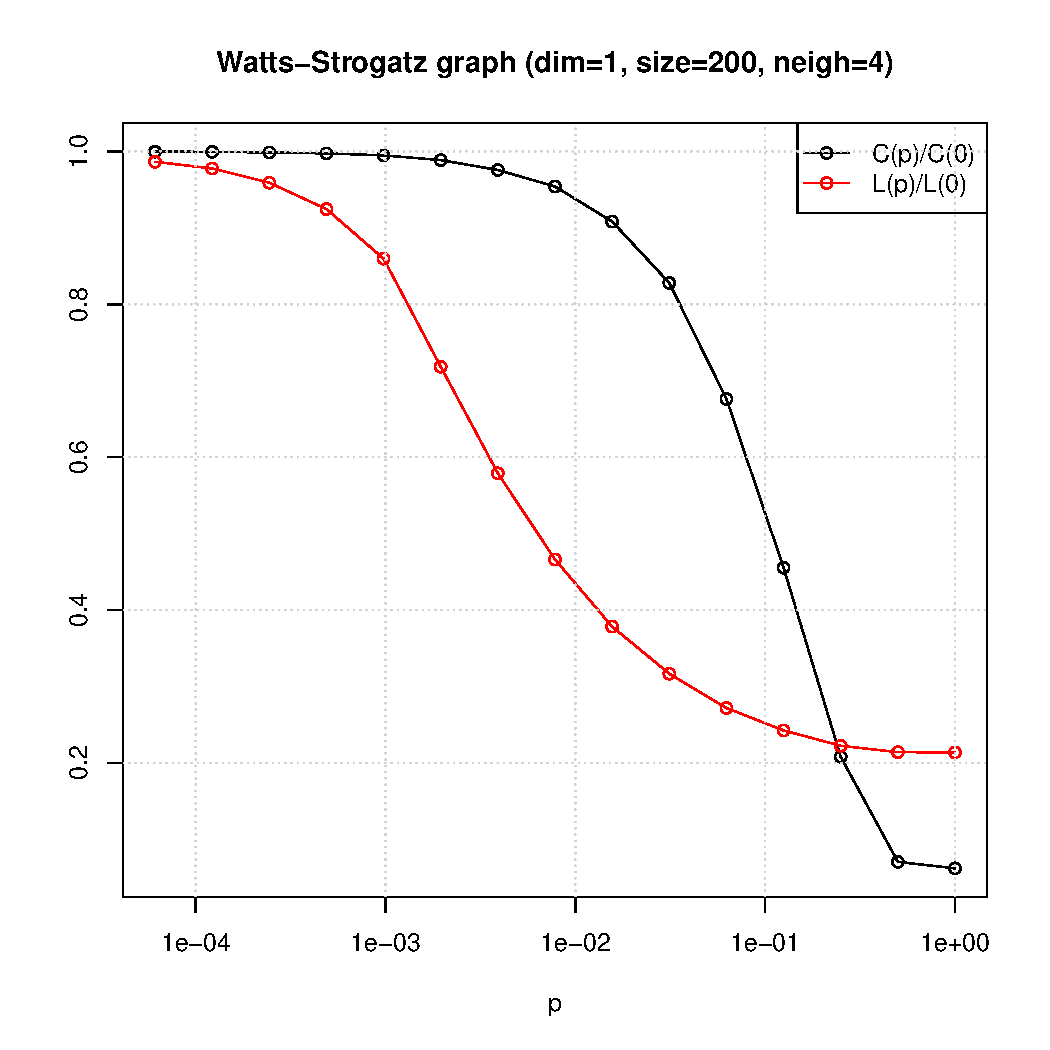
\includegraphics[width=.8\textwidth]{ws.pdf}
\end{center}

\newpage
\section{Erdös--Rényi model}

The probability $p$ of connecting two vertex is set to $p = (1+\epsilon) 
\ln(n)/n$ to keep the graph connected with high probability. In order to find a 
good $\epsilon$ value, a set of random graphs are generated, with values of 
$\epsilon \in [0.4, 0.6]$. The edge connectivity $e$ is measured in a set of 
$r=2000$ runs. The relative number of graphs with $e = 0$ is plot against 
$\epsilon$ in the figure \ref{fig:zeros} and the mean of $e$ is plotted in 
\ref{fig:mean}.
%
\begin{figure}[htp]
%	\centering
	\subfloat[The relative number of disconnected graphs against $\epsilon$]{%
		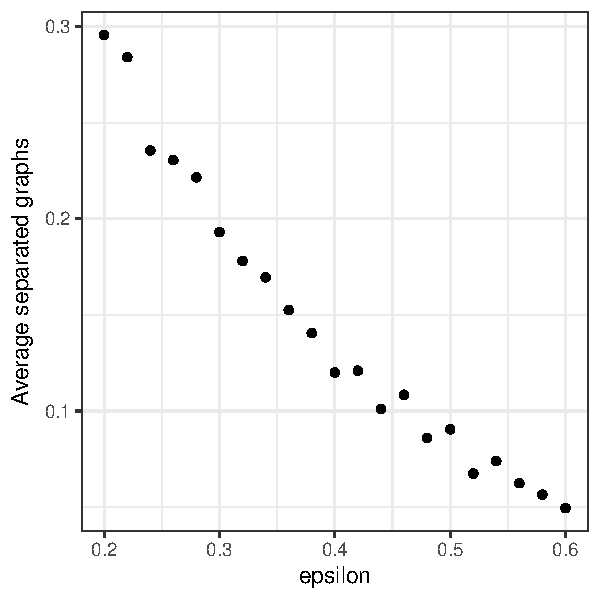
\includegraphics[width=0.48\textwidth]{er-zeros.pdf}%
		\label{fig:zeros}%
	}%
	\hfill%
	\subfloat[The mean of edge connectivity for graphs with different 
	$\epsilon$]{%
		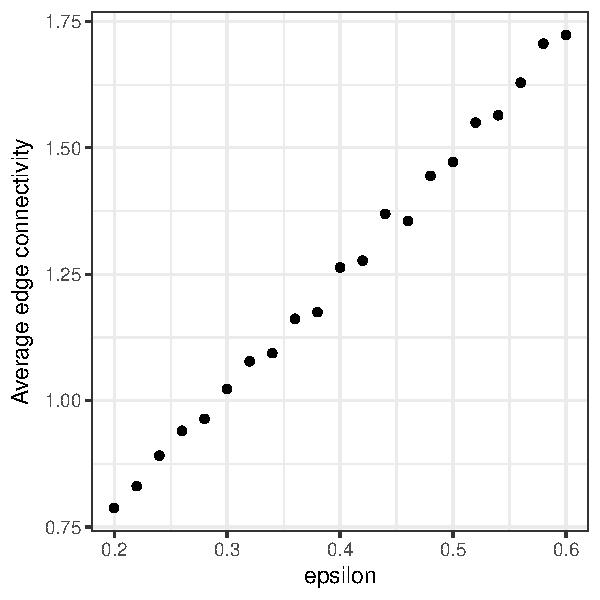
\includegraphics[width=0.48\textwidth]{er-prob.pdf}%
		\label{fig:mean}%
	}%
\end{figure}

The chosen value of $\epsilon = 0.5$ keeps the number of disconnected graphs 
close to 10\%, while the mean edge connectivity is close to $1.5$. Finally, the 
average shortest path is ploted against the number of nodes $n$ of a 
Erdös--Rényi graph. The mean values of 10 random graphs are computed to reduce 
the variance. The number of nodes is set up to 5000, to maintain a reasonable 
computing time.
%
\begin{center}
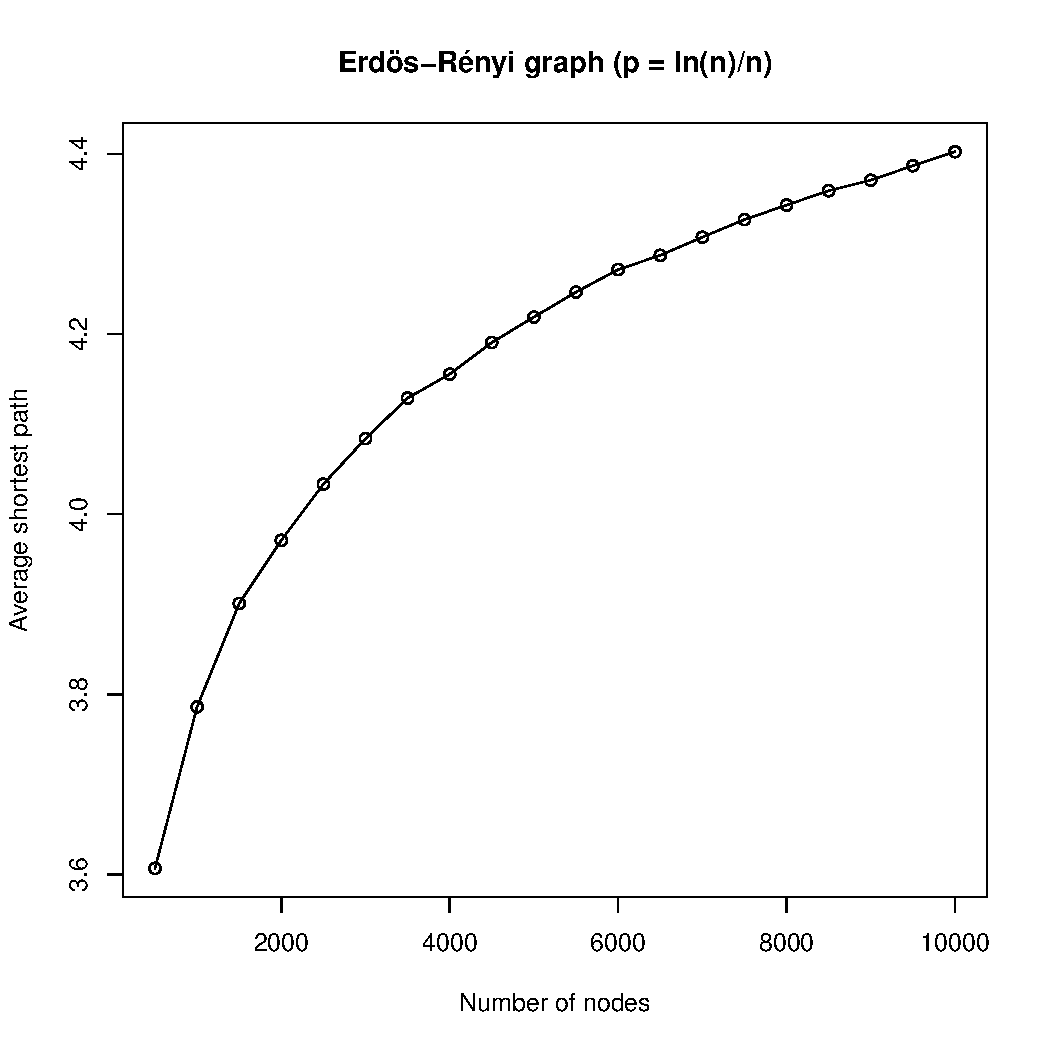
\includegraphics[width=0.5\textwidth]{er.pdf}
\end{center}

\end{document}
